Within this chapter the general design of the system that will be implementing the new process is described. First of all the general design is discussed, followed by an explanation about the used languages and frameworks. Finally, the rule set request is explained. 

\section{General Design}
Due to the fact that the system should be a web application, a modified \gls{mvc} is used to split up business logic and the user interface presentation. The system has the following components:

%\begin{table}[h!]
	\begin{longtable}{|p{4cm}|p{11cm}|} \hline
		\rowcolor{Gray}Component & Functionality \\ \hline
		View & Presents the result of the  business logic and triggers the user interaction.\\ \hline
		Controller & Handles the communication between view and service in such a way, that the other components do not need to know from each other. The controller processes all transmitted actions from the view and requests the service for the corresponding tasks. The returned information is prepared for the view and presented through the view to the user. \\ \hline
		Service & This component holds the business logic of the system and coordinates the interactions with the information components. In the standard \gls{mvc} this responsibility is held by the controller, the service is introduced to offload this functionality.\\ \hline
		Model & Inside the model the information are stored, which are exchanged between all components.\\ \hline
		\Gls{erp} Connector & It is responsible for the communication with the \gls{erp}. It has to provide information about documents, customer and the employee that uploaded the document. \\ \hline
		Signing Tool Connector & At this component the signing process of a selected document is managed. Therefore, information about the signers are required and the document file. \\ \hline
		User Reader & This component handles user and employee data from the company. It is responsible for the login to the system and should store all members of the company with their position. The required information are name, position, phone number and mail address, because they are either needed to give the information, who had to sign a document together with the user based on the rule set. Additionally, it has the responsibility to pass the required signer information directly to the signing tool. \\ \hline
		Rules Reader & An important component is the rules reader, because it knows the signing guideline of the company. It provides for the system the information which company positions had to sign a document based on its type, value and the user that initiated the signing process.\\ \hline
		\caption{System Components}
		\label{tab:listingSystemComponents}
	\end{longtable}
%	\centering
%	\caption{Listing of Systems Components}
%	\label{tab:listingSystemComponents}
%\end{table}

In figure \ref{fig:generalDesign} the communication between the components is visualized.
In the case the arrows have the description ``exchange'', the two connected components transfer information and trigger actions. If the description is ``use'', the component the arrow points at is used as a data storage that is transmitted between other components and only stores information.  The description ``act'' means that the user can manipulate this component to reach his aims with the system. \newline
As can be seen the center of the communication is the service component. This corresponds with its functionality to make the complete business logic. Also the model component is only marked as ``used'' from the other components. That is also explained by its functionality as data storage.  

\begin{figure}[h!]
	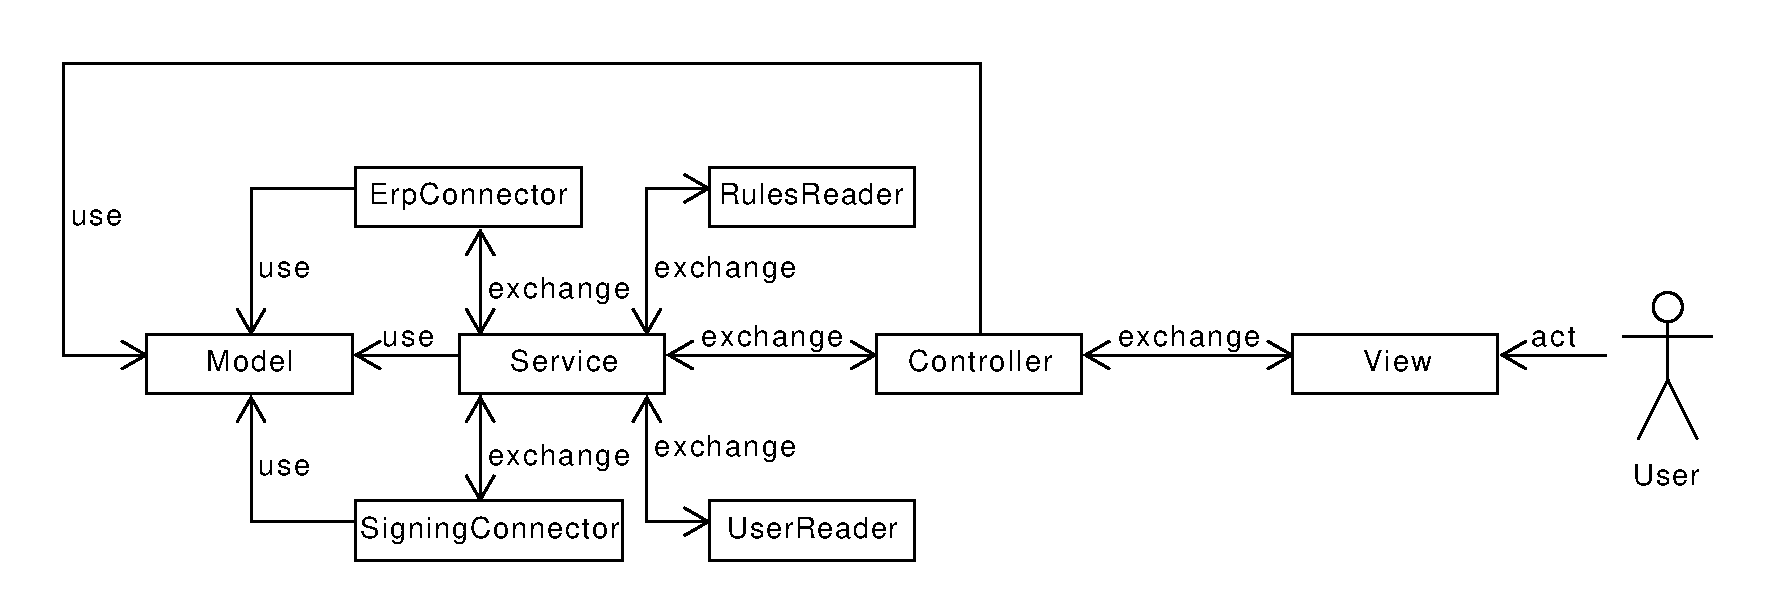
\includegraphics[width=\linewidth]{./design/images/generalCommunication.pdf}
	\centering
	\caption{General system design}
	\label{fig:generalDesign}
\end{figure}

Due to the fact that it is unclear which \gls{erp} will be used and that therefore no decision is made for a signing tool, the connector components should be as variable as possible to be independent from the later tools. That leads to the design decision to define interfaces for those connectors, which are implemented with mocked systems to present the process. \newline
Beside these interfaces, two more should be created for the reader components, because those have connections to the data storages, these depend on which company is using the system later on. In most cases they already have an authentication system, that also stores the position of the company members. When implementing the rules reader, the preferences of the later administrators are important, because they are responsible to maintain the data, if changes are made to the signing guideline. Therefore, it is important that they can choose a preferred way to store the data. Following this, the interfaces are explained in more detail.

\subsection*{Enterprise Resource Planning System Connector}
This interface defines the methods for receiving information of documents from the \gls{erp}, the document file itself and the storing of the signed document. Therefore the search functionality is especially important for this interface. In general a lot of documents are stored inside an \gls{erp} and it is not possible to present them all in a simple overview. At the moment, it should be possible to search for the following information: document type, document name, related customer name and the name of the employee, who created and stored the document inside the \gls{erp}.

\subsection*{Rule Reader}
Within this interface only one method is defined, to get the information which combinations of company members have the right to sign the selected document. It will receive the information about the type of document, the value of the document and the position of the user that wants to sign the document. The implementation always follows the request described in section \ref{sec:ruleRequest}.

\subsection*{Signing Tool Connector}
This component is responsible for the connection to the signing tool. It has the task to pass all required information for the signing and the document to the tool. Therefore one method exists, which gets that required data inside a container and returns a true or false status when everything goes well or an error occurs. \newline
Furthermore, another task exists: To collect signed documents based on their name. This is done within another method, which gets the name of the document and returns a container with all information belonging to the signed document. In the case, that the document is not signed, an empty container should be returned. 

\subsection*{User Reader}
Inside this interface different functionalities are defined, which are split up in the areas: position groups and employee information. In the first area the implementation provides the information which employees have a certain position at the company. The second area is responsible for giving specific information about a employee. These information are company position, mail address and phone number.

\section{Used Programming Language and Frameworks}
At the start of the implementation a discussion was held, which programming language to use. Available were several options, due to the usage of \textit{DocuSign eSign} for mocking the signing tool. It provides different \glspl{sdk} for C\#, Node.js and Java \parencite{docusign2018sdk}, as well as a \gls{rest} \gls{api}. The choice was Java, because it is one of the standard programming languages of \gls{cc} and mostly well known by other programmers. Due to the fact that there were time issues at the end of the project, this language was selected.

Another decision was to use \textit{Maven}, because it builds the complete dependencies from the project independently from the \gls{os}. That is useful for automated testing in pipeline systems and deploying. \newline
The decision was made to use \textit{Spring Boot}. With this tool it is simple to setup a project without the need to install a server and deploy a \gls{db}. This is beneficial for prototyping, which should be made in this project. Furthermore, it was possible to gather new experiences with the framework and an approach for the bachelor thesis is to get new experiences. Additionally, \textit{Spring Boot} provides functionalities for security and \gls{mvc} applications, which are needed in the project. \newline
All other used tools and frameworks are listed in table \ref{tab:frameworks}.

\begin{table}[h!]
	\begin{tabular}{|p{2cm}|p{13cm}|} \hline
		\rowcolor{Gray}Framework/ Tool & Functionality \\ \hline
		Lombok & Project Lombok is an open source Java library that generates simple code (e.g. Getter and Setters) based on set annotations \parencite{lombok2018}. It is used to simplify the implementation and make the code structure more clean. \\ \hline
		Mockito & Provides functionalities to mock classes and helps to test logic independent from the implementation \parencite{mockito2018}. This functionality is used to test the logic independently from the data storages used in the proof-of-concepts. \\ \hline
		H2 & This is a lightweight \gls{sql} \gls{db} with an already existing \gls{api} for data transferring between system and \gls{db}. Furthermore, it is developed based on the programming language Java. \parencite{hs2018} Inside an H2 \gls{db} the rule set will be stored. \\ \hline
		JUnit & This framework provides a lot of functionalities for testing like test suites or specific annotations for testing \parencite{junit2018}. \\ \hline
		Thymeleaf& A template engine for web applications to easily exchange data from \textit{Hypertext Markup Language} files with \textit{Java} classes \parencite{thymeleaf2018}. Specifically usable for the \gls{mvc}.  \\ \hline
	\end{tabular}
	\centering
	\caption{Used Frameworks}
	\label{tab:frameworks}
\end{table}

\section{Rule Set Request}\label{sec:ruleRequest}
Inside the rule set the signing guideline is stored for the system. In general it can be said that there exist four general data sets:
\begin{itemize}
	\item Company positions: \newline
	Inside this data set all the positions of a company are listed. Each of them has different rights and liabilities.
	\item Document types: \newline
	At a company several different document types exist and they need to be handled differently regarding the signatures. 
	\item Value ranges: \newline
	In a signing guideline several different value ranges are listed. They are inserted in this data set. Each of them has a minimum value and a maximum value.
	\item Signing groups: \newline
	Inside a company several signing groups exists, which consist of different company positions. Each group has combined rights.
\end{itemize}

The rule set is a combination of the previously explained data sets. It defines for each document type and the corresponding value ranges which signing group is allowed to sign the combination. \newline
In the situation a user selects a document for signing, the system needs to analyze based on the document type, the value of the document and the position of the user. If the user is allowed to sign at all, it has to be checked if there are other company positions that need to sign along. 

The mathematical presentation of this request is presented in the appendix \ref{mathCode}. The following figure \ref{fig:visualizationRuleRequest} visualize the process.
\begin{figure}[h!]
	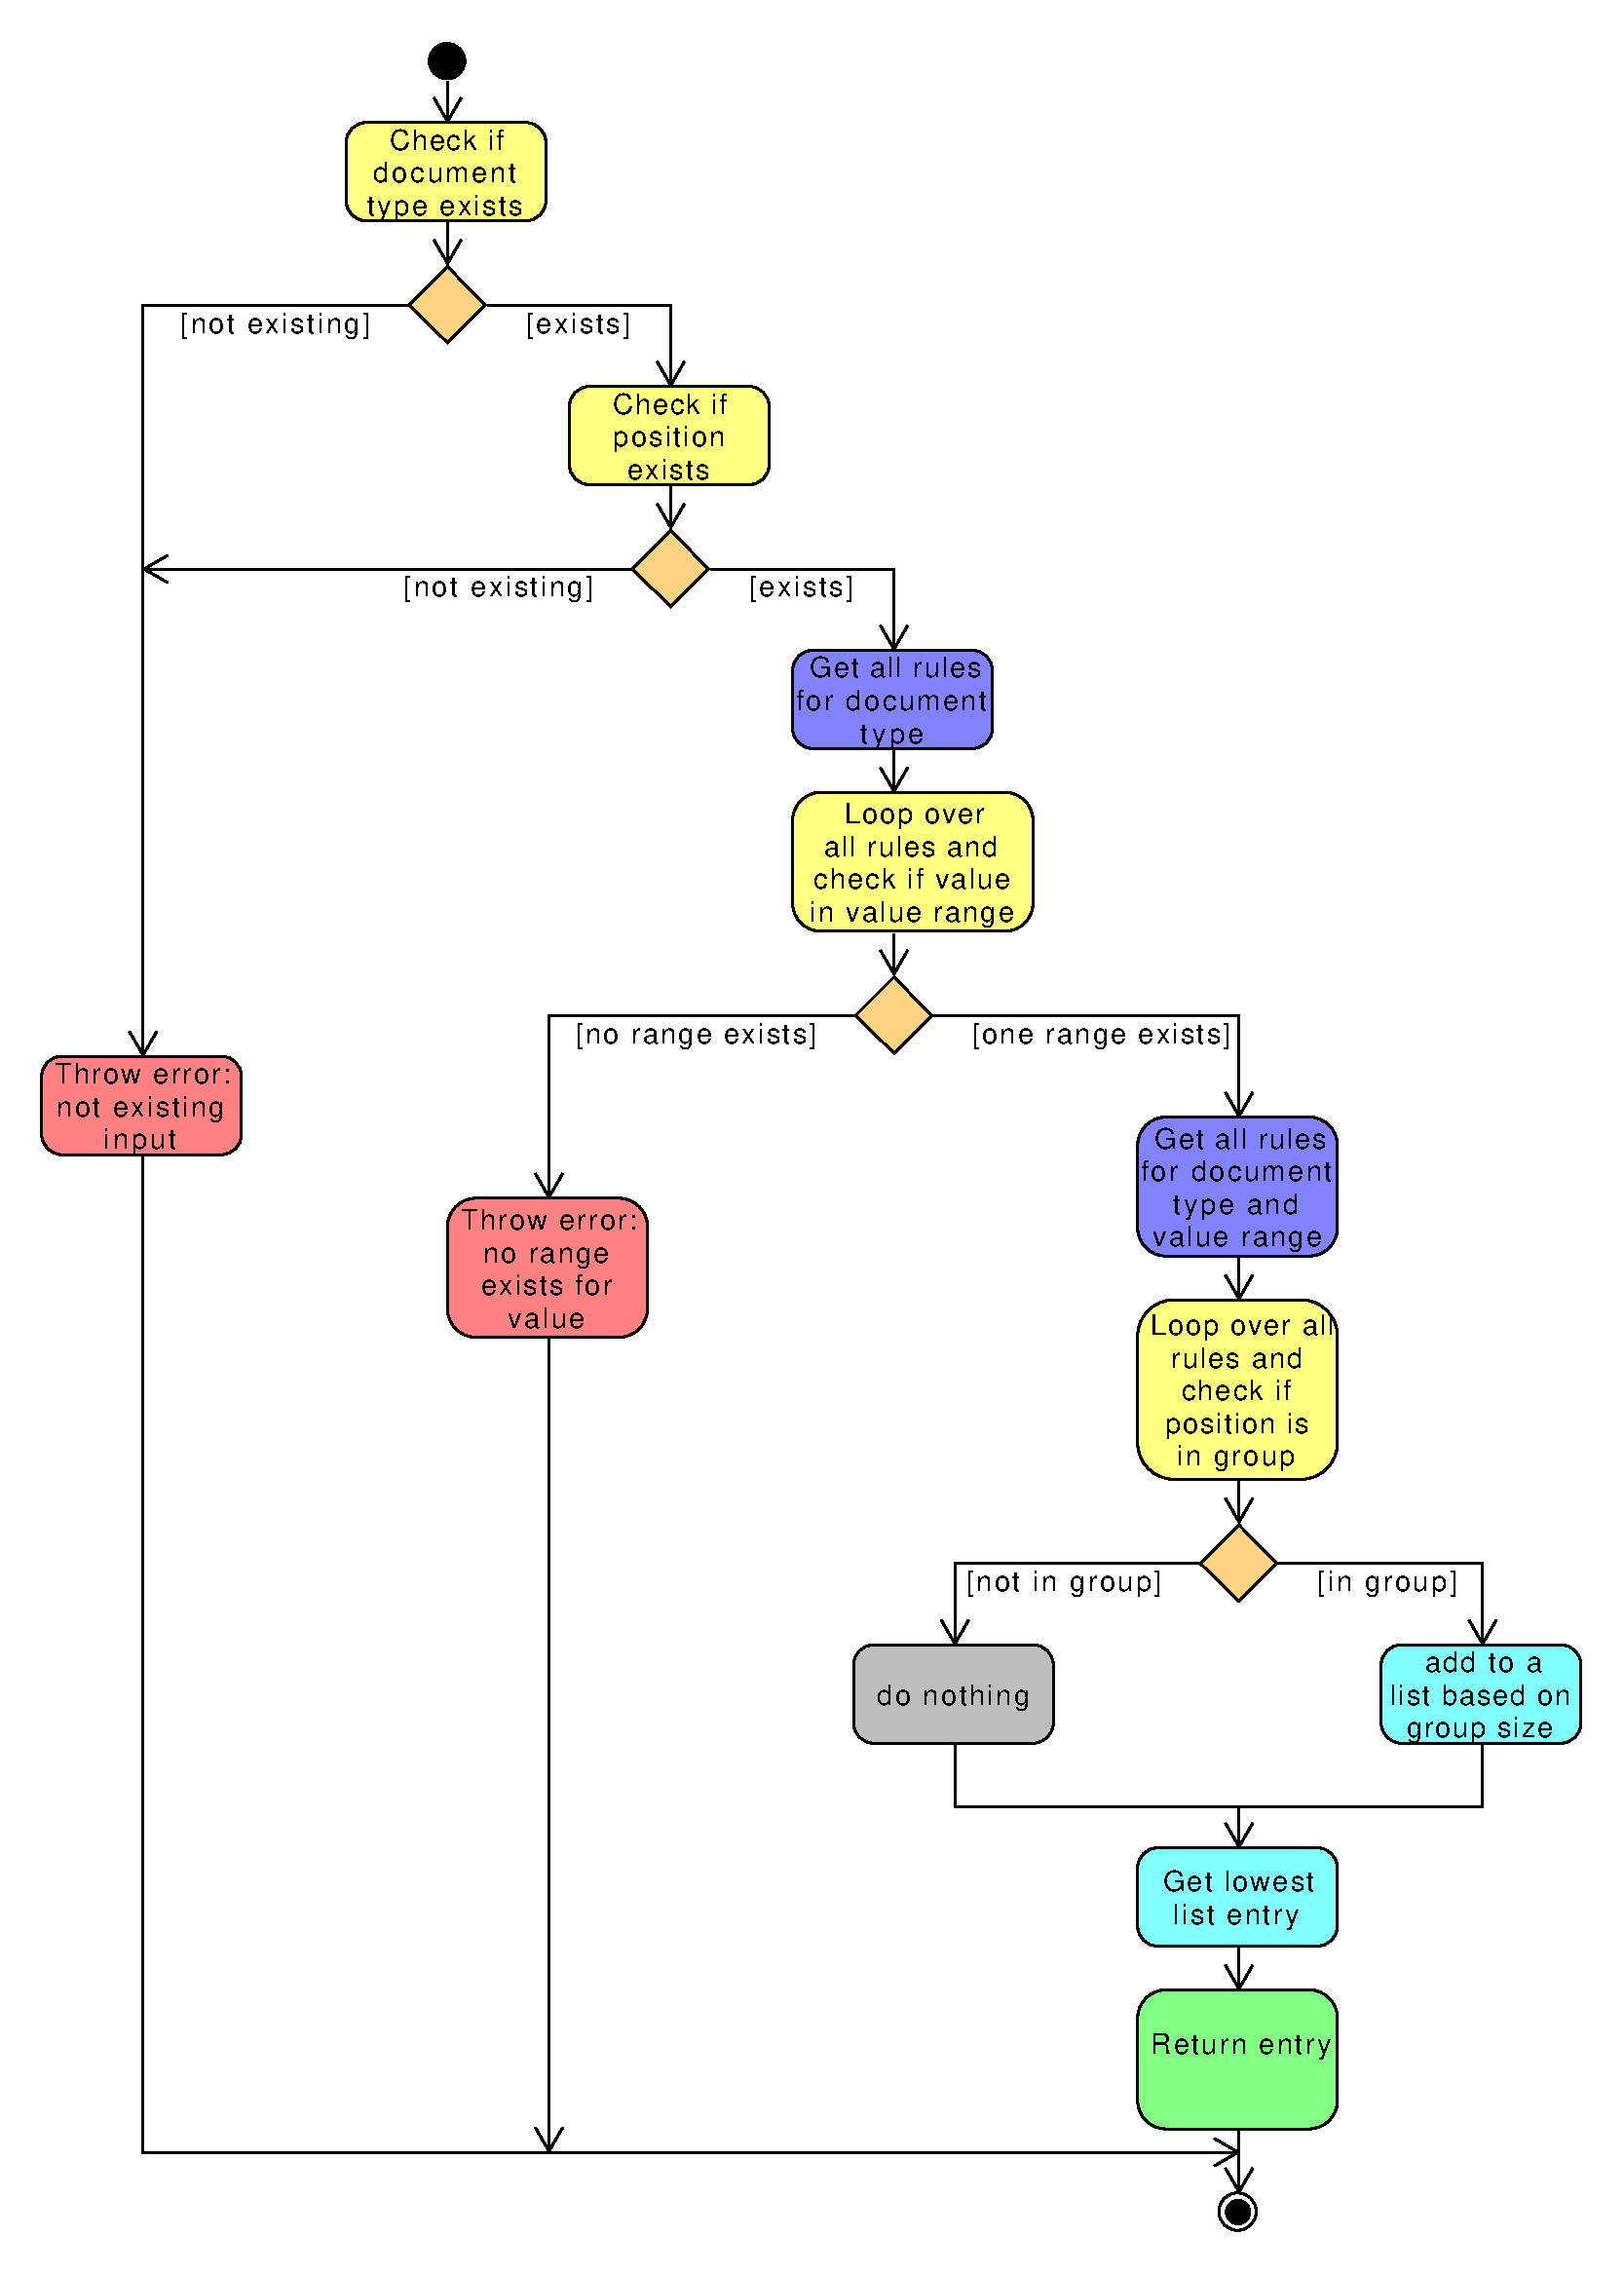
\includegraphics[width=0.8\linewidth]{./design/images/activityRuleSetRequest.pdf}
	\centering
	\caption{Process of rule set request}
	\label{fig:visualizationRuleRequest}
\end{figure}
In the first instance it has to be checked that both the document type and the position exist inside the data sets, otherwise an exception is to be thrown that informs the system about the invalid information. Next all rules regarding the specific document type should be collected from the rule set data. Inside this, the different value ranges need to be fetched. For each of these value ranges, the minimum and maximum are gathered and it is checked if the given value for the request is between those two. If there is no match an information is given to the system via an exception. Else all signing groups from the rule set with the specific document type and value range are called and it will be proofed whether the use position is inside this group or not. In the situation, that the position of an employee is inside the signing group, the system should add the signing group to a list based on the group size. If the user is not in the group, nothing should happen. Finally, the groups with the smallest size should be returned. In the scenario that there is no signing group at all, an empty list should be returned, which signalizes that the user does not have the permission to sign the document based on the signing rule set. 

\subsection*{Example}
For a better understanding an example is given based on the signing guideline from \gls{cc} presented in table \ref{tab:newSigningGuideline}: \newline
The general data sets:
\begin{itemize}
	\item Company positions: employee; salesman; manager; procurator; chairman
	\item Document types: quotation; \gls{nda}; contract
	\item Value ranges: 0 - 50 000; 50 000,01 - 400 000; 400 000,01 - $\infty$; 0 - $\infty$
	\item Signing groups (extracts): employee only; manager only; salesman with manager; manager with chairman; ....
\end{itemize}

For the rule set example an extract is selected. In the following the entries are presented:
\begin{enumerate}
	\item Contract; (0 - 50 000); salesman alone
	\item Contract; (0 - 50 000); manager alone
	\item Contract; (0 - 50 000); chairman alone
	\item Contract; (50 000,01 - 400 000); salesman with manager
	\item Contract; (50 000,01 - 400 000); salesman with chairman
	\item Contract; (50 000,01 - 400 000); manager alone
	\item Contract; (50 000,01 - 400 000); chairman alone
	\item Contract; (400 000,01 - $\infty$); salesman with chairman
	\item Contract; (400 000,01 - $\infty$); manager with chairman
	\item Contract; (400 000,01 - $\infty$); chairman alone
\end{enumerate}